%-----------------------------------------------
% Dateiname: CreateQueryObjects.tex
% Autor    : Stefano Kowalke <blueduck@gmx.net>
% Lizenz   : BSD
%-----------------------------------------------
\section{Umstellen der Query-Methoden auf Doctrine DBAL und Prepared Statements}
\label{prototype:sec:usingDoctrinePreparedStatements}

In Kapitel~\ref{sec:currentSituation} zur Datenbank API wurde bereits die Unterteilung in Generierende und Ausführende SQL-Methoden erläutert. Die Generierung der Abfrage erfolgt anhand der Parameter, die – zusammen mit den entsprechenden SQL-Abfragen – in eine Zeichenkette umgewandelt und zurückgegeben werden.

\begin{listing}[H]
\begin{phpcode}
public function UPDATEquery(
  $table,
  $where,
  array $fields_values,
  $no_quote_fields = FALSE
  ) {
  ...
    $fields = array();
	if (is_array($fields_values) && count($fields_values)) {
	  // Quote and escape values
	  $nArr = $this->fullQuoteArray(
	            $fields_values,
	            $table,
	            $no_quote_fields,
	            TRUE
	          );
	  foreach ($nArr as $k => $v) {
	    $fields[] = $k . '=' . $v;
	  }
	}

	$query = 'UPDATE ' . $table . ' SET ' . implode(',', $fields) .
		((string)$where !== '' ? ' WHERE ' . $where : '');
	...
	return $query;
  }
}
\end{phpcode}
\caption{Original UPDATEquery der alten Datenbank API}
\label{lst:UPDATEoldAPI}
\end{listing}

Doctrine DBAL bietet mit dem \phpinline{QueryBuilder} eine Klasse an, mit der die Formulierung von SQL-Abfragen abstrahiert werden kann. Die Generierung der SQL-Abfrage aus Listing~\ref{lst:UPDATEoldAPI} konnte durch die Nutzung des \phpinline{QueryBuilders} wie folgt verändert werden:

\begin{listing}[H]
\begin{phpcode}
public function UPDATEquery(...) {
...
  $query = $this->link->createQueryBuilder()
    ->update('pages')
    ->set('title', 'Foo')
    ->where('id = 1')
    ->getSQL();
...
}
\end{phpcode}
\caption{Generierung der SQL-Abfrage wird an den QueryBuilder delegiert}
\label{lst:createSqlByDirectCallToQueryBuilder}
\end{listing}

Dies wurde für alle generierenden Methoden der alten API realisiert. Dabei wurde der Code der Methoden in die neue API kopiert, während die alten Klassen den Aufruf an ihre Elternmethode delegieren \phpinline{return parent::insertQuery(...)}. Dies wurde notwendig, da der Methodenname der alten API nicht der \gls{cgl} entsprach; der Aufruf über \phpinline{parent::} und nicht über \phpinline{$this->} wurde notwendig, da \gls{php} nicht zwischen Groß- und Kleinschreibung unterscheidet - die Methoden \phpinline{INSERTquery()} und \phpinline{insertQuery()} werden als identisch angesehen.

Durch diesen Schritt wurde die letzte Abhängigkeit zu einem bestimmten \gls{dbms} aufgelöst.

Während die alte Datenbank API wie gewohnt benutzt werden kann (siehe Listing~\ref{lst:resetStageOfElementsOldAPI}), wird für die neue Datenbank API eine Abstraktion zur Formulierung von SQL-Abfragen nach dem Vorbild des \phpinline{QueryBuilders} angestrebt (siehe Listing~\ref{lst:resetStageOfElementsNewAPI}). Wie zu sehen ist, werden dort auch die logischen Ausdrücke abstrahiert.

\begin{listing}[H]
\begin{phpcode}
protected function resetStageOfElements($stageId) {
  $fields = array('t3ver_stage' =>
    \TYPO3\CMS\Workspaces\Service\StagesService::STAGE_EDIT_ID);
  foreach ($this->getTcaTables() as $tcaTable) {
    if (BackendUtility::isTableWorkspaceEnabled($tcaTable)) {
      $where = 't3ver_stage = ' . (int)$stageId;
      $where .= ' AND t3ver_wsid > 0 AND pid=-1';
      $GLOBALS['TYPO3_DB']->exec_UPDATEquery($tcaTable, $where, $fields);
    }
  }
}
\end{phpcode}
\caption{}
\label{lst:resetStageOfElementsOldAPI}
\end{listing}

\begin{listing}[H]
\begin{phpcode}
protected function resetStageOfElements($stageId) {
  ...
      $dbh = $GLOBALS['TYPO3_DB'];
      $expr = $dbh->expr();
      $query = $dbh->createUpdateQuery();

      $query->update($tcaTable)
        ->set(
          't3ver_stage',
          \TYPO3\CMS\Workspaces\Service\StagesService::STAGE_EDIT_ID)
        ->where(
          $expr->equals(t3ver_stage, $stageId),
          $expr->greaterThan(t3ver_wsid, 0),
          $expr->equals(pid, -1)
        )
      );

      $query->execute();
 ...
}
\end{phpcode}
\caption{Ausblick auf die fertige Query-API}
\label{lst:resetStageOfElementsNewAPI}
\end{listing}

Es wurde darauf verzichtet die API des \phpinline{QueryBuilder} direkt anzubieten. Die Gründe dafür sind

\begin{itemize}
\item vereinfachte API: ein \phpinline{Query}-Objekt bietet lediglich die für seine Domain notwendigen Methoden an. Dadurch kann es auch nicht zur Formulierung von syntaktisch falschen Abfragen kommen.
\item keine Abhängigkeit zu Doctrine DBAL: die Implementation der Methoden kann – wie am Anfang des Kapitels gezeigt - jederzeit gegen etwas anderes ausgetauscht werden.
\end{itemize}

Zur Umsetzung wurde das \textit{Facade}-Entwurfsmuster angewendet. Hier stellt ein Domain-spezifisches \phpinline{Query}-Objekt die \textit{Fassade} dar und bietet nach außen lediglich eine Teilmenge der von \phpinline{QueryBuilder} zur Verfügung gestellten Methoden.

\begin{figure}[H]
    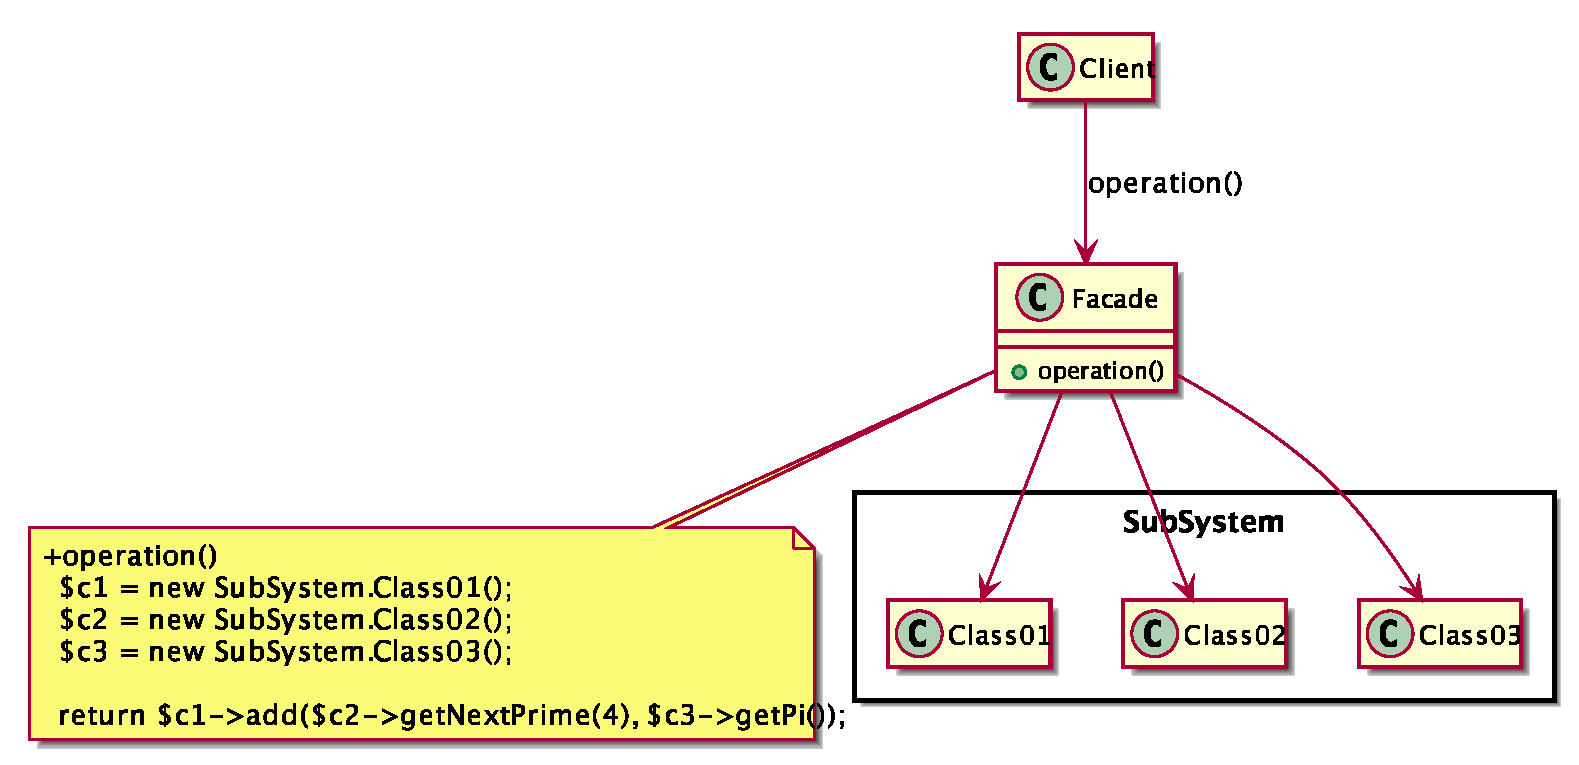
\includegraphics[scale=0.5]{gfx/uml/FacadePattern.eps}
    \caption{Schematischer Aufbau des Fassade-Entwurfsmusters}
    \label{fig:facadePattern}
\end{figure}

Das folgende UML-Diagramm zeigt anhand der \phpinline{TruncateQuery}- und \phpinline{UpdateQuery}-Objekte die fertige Hierachie. Die Wurzel stellt das \phpinline{QueryInterface} dar, in dem alle Methoden festgelegt worden sind, die von allen \phpinline{Query}-Objekten implementiert werden müssen. Dadurch wird sichergestellt, dass jedes \phpinline{Query}-Objekt in Verbindung mit PreparedStatements verwendet werden kann und die Kenntnis darüber besitzt wie es in eine \gls{sql}-Abfrage konvertiert und ausgeführt werden kann.

Das Interface wird um ein Interface erweitert, welches die Domain-spezifischen Methoden festlegt. So muß ein \phpinline{TruncateQuery} die Methoden \phpinline{truncate()}, \phpinline{getType()} und \phpinline{getSql()} implementieren. Die anderen vorgeschriebenen Methoden werden von der Klasse phpinline{AbstractQuery} implementiert, die von jeder \phpinline{Query}-Klasse erweitert wird.

\begin{figure}[H]
    \centering
    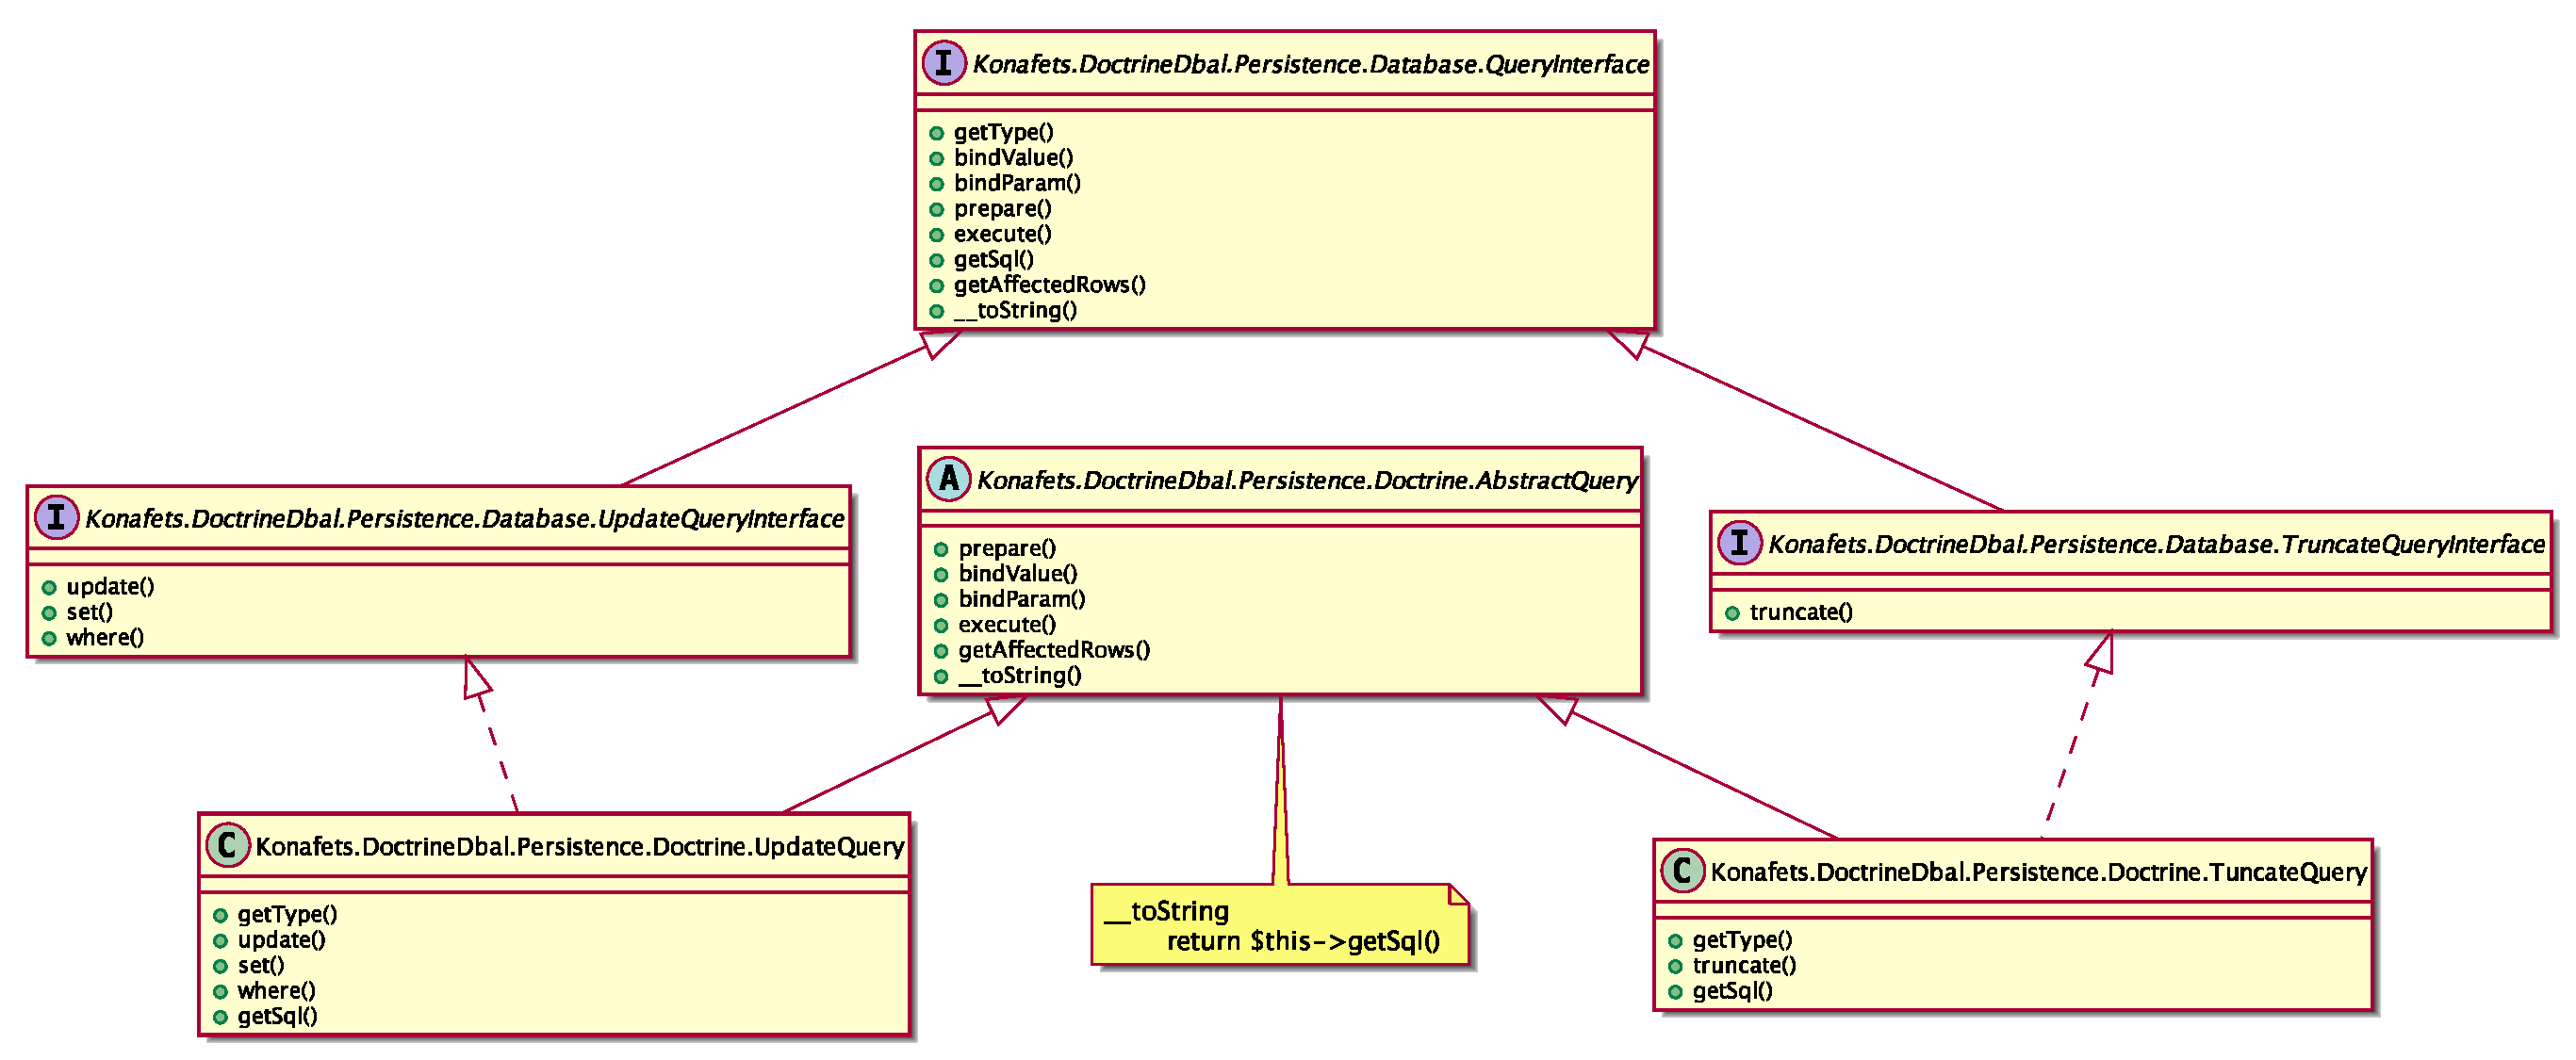
\includegraphics[scale=0.5, angle=90]{gfx/uml/NewAPI/UpdateQuery.eps}
    \caption{Aufbau der Query-API}
    \label{fig:newQueryAPI}
\end{figure}

Der Aufbau ist an die Implementation der Datenbank API von EzPublish angelehnt, die von Benjamin Eberlei eingeführt wurde.\footnote{\url{http://bit.ly/ezpublish-database-api}} Während die Erzeugung der \gls{sql}-Abfragen innerhalb der EzPublish Datenbank API manuell erfolgt, delegieren die Methoden der \phpinline{Query}-Klassen des Prototypen den Aufruf an den \phpinline{QueryBuilder}.

\begin{listing}[H]
\begin{phpcode}
public function update($table) {
  $this->queryBuilder->update($table);

  return $this;
}

public function set($columns, $values) {
  $this->queryBuilder->set($columns, $values);

  return $this;
}

public function where() {
  $constraints = func_get_args();
  $where = array();

  foreach ($constraints as $constraint) {
    if ($constraint !== '') {
	  $where[] = $constraint;
	}
  }

  if (count($where)) {
    call_user_func_array(array($this->queryBuilder, 'where'), $where);
  }

  return $this;
}

public function getSql() {
  return $this->queryBuilder->getSQL();
}
\end{phpcode}
\caption{Die Konvertierung des UpdateQuery erfolgt über den QueryBuilder}
\label{lst:getSqlMethodOfUpdateQuery}
\end{listing}

Der Klasse \phpinline{\Konafets\DoctrineDbal\Persistence\Doctrine\DatabaseConnection} wurden \phpinline{create*Query()}-Methoden hinzugefügt, die die Instantiierung eines \phpinline{Query}-Objekts vereinfachen.

\begin{listing}[H]
\begin{phpcode}
public function createUpdateQuery() {
  if (!$this->isConnected) {
    $this->connectDatabase();
  }

  return GeneralUtility::makeInstance(
  		  '\\Konafets\\DoctrineDbal\\Persistence\\Doctrine\\UpdateQuery',
  		  $this->link
  		);
}
\end{phpcode}
\caption{Die Erzeugung eines UpdateQuery-Objekts}
\label{lst:createUpdateQuery}
\end{listing}

Nun konnte die Abhängigkeit zu Doctrine DBAL durch den direkten Aufruf des \phpinline{QueryBuilders} aus Listing~\ref{lst:createSqlByDirectCallToQueryBuilder} entfernt werden:

\begin{listing}[H]
\begin{phpcode}
public function UpdateQuery(...) {
...
  $query = $this->createUpdateQuery()
    ->update('pages')
    ->set('title', 'Foo')
    ->where('id = 1')
    ->getSQL();
...
}
\end{phpcode}
\caption{}
\label{}
\end{listing}

Zur Abstraktion der logischen Ausdrücke aus dem Codebeispiel~\ref{lst:resetStageOfElementsNewAPI} wurde die Klasse \phpinline{Expression} implementiert, die ebenfalls eine Fassade darstellt - dieses Mal vor der Klasse \phpinline{\doctrine\DBAL\Query\ExpressionBuilder}. Das Namensschema folgt der Extbase-\gls{api}.

\begin{figure}[H]
    \centering
    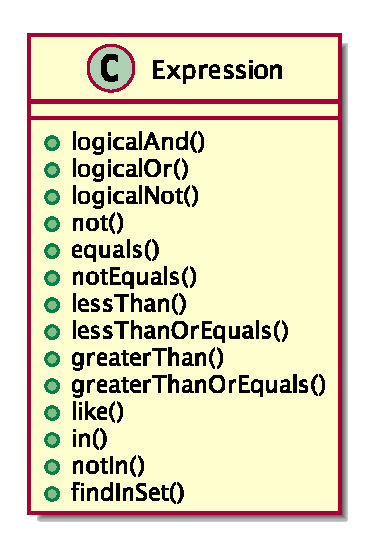
\includegraphics[scale=0.5]{gfx/uml/NewAPI/Expression.eps}
    \caption{Die Klasse Expression}
    \label{fig:expressionClass}
\end{figure}

Die Query-API kann nun, wie es in Listing~\ref{lst:resetStageOfElementsNewAPI} gezeigt, verwendet werden.

Aus der Datei \pdf{typo3/sysext/core/Classes/Authentication/AbstractUserAuthentication.php} wurde die Methode \phpinline{fetchUserSession()} ausgewählt. An ihr soll die Migration der alten API auf die neue API unter Verwendung des \phpinline{UpdateQuery} gezeigt werden. Die Methode aktualisiert die Session für den angemeldeten Backendbenutzer und wird bei jedem Aufruf des Backends aufgerufen. Dadurch ist ist sehr gut überprüfbar, ob die Migration wie erwartet funktioniert. Die Methode erzeugt folgende SQL-Abfrage: \\

\begin{listing}[H]
\begin{mysqlcode}
UPDATE be_sessions
SET ses_tstamp = '1400788819'
WHERE ses_id='c2c75…'
AND ses_name='be_typo_user'
\end{mysqlcode}
\caption{Die von fetchUserSession erzeugte SQL-Abfrage}
\label{lst:fetchUserSqlQuery}
\end{listing}

Die Werte in der \mysqlinline{WHERE}-Bedingung werden durch \phpinline{fullQuoteStr()} maskiert, um SQL-Injections zu verhindern.

\begin{listing}[H]
\begin{phpcode}
public function fetchUserSession($skipSessionUpdate = FALSE) {
...
  if ($timeout > 0 && $GLOBALS['EXEC_TIME'] < $user['ses_tstamp'] + $timeout) {
    if (!$skipSessionUpdate) {

	  $this->db->exec_UPDATEquery(
	    $this->session_table,
	    'ses_id=' . $this->db->fullQuoteStr(
	      $this->id,
	      $this->session_table
	    ) .
	      ' AND ses_name=' . $this->db->fullQuoteStr(
	        $this->name,
	        $this->session_table
	      ),
	    array('ses_tstamp' => $GLOBALS['EXEC_TIME']));

	  // Make sure that the timestamp is also updated in the array
	  $user['ses_tstamp'] = $GLOBALS['EXEC_TIME
	}
  } else {
    // Delete any user set...
	$this->logoff();
  }'];
…
}
\end{phpcode}
\caption{fetchUserSession() im Original}
\label{lst:fetchUserSessionBeforeMigration}
\end{listing}


Das folgende Listing zeigt den gleichen Code nach der Migration. Obwohl die Methoden bereits weiter oben vorgestellt wurden, soll hier auf die Verwendung eines \phpinline{FluentInterfaces} hingewiesen werden. Dies ermöglicht zum einen die Verkettung der Methoden und zum anderen eine lesbare API, bei der auf den ersten Blick der Kontext eines jeden Parameters anhand des Methodennamens deutlich wird. Realisiert werden \phpinline{Fluent Interface} durch die Zurückgabe des eigenen Objekts in der Methode mittels \phpinline{return $this}.

\begin{listing}[H]
\begin{phpcode}
 ...
  if ($timeout > 0 && $GLOBALS['EXEC_TIME'] < $user['ses_tstamp'] + $timeout) {
    if (!$skipSessionUpdate) {

      $query = $this->db->createUpdateQuery();
      $query->update($this->session_table)
        ->set('ses_tstamp', $GLOBALS['EXEC_TIME'])
        ->where(
          $query->expr->equals('ses_id', $this->db->quote($this->id)),
          $query->expr->equals('ses_name', $this->db->quote($this->name))
        )->execute();
	}
  } else {
    // Delete any user set...
	$this->logoff();
  ();}
...
)
\end{phpcode}
\caption{fetchUserSession() nach der Migration mit manueller Maskierung}
\label{lst:fetchUserSessionAfterMigration}
\end{listing}

Auch hier wurde die Maskierung manuell durch \phpinline{DatabaseConnection::quote()} vorgenommen. In Kapitel~\ref{basics:doctrine:subsubsec:preparedStatements} wurde auf die Gefahren von SQL-Injections hingewiesen und wie diese durch Prepared Statements (siehe Kaptiel~\ref{basics:doctrine:subsubsec:preparedStatements}) verhindert werden können. Das nächste Listing zeigt wie diese mit der API genutzt werden können.

\begin{listing}[H]
\begin{phpcode}
$query = $this->db->createUpdateQuery();
$query->update($this->session_table)
  ->set('ses_tstamp', $GLOBALS['EXEC_TIME'])
  ->where(
    $query->expr->equals('ses_id', $query->bindValue($this->id)),
    $query->expr->equals('ses_name', $query->bindValue($this->name))
  )->execute();
}
\end{phpcode}
\caption{fetchUserSession() in Verbindung mit PreparedStatements}
\label{lst:fetchUserSessionAfterMigrationPreparedStatements}
\end{listing}


Die Methode \phpinline{quote()} wurde gegen \phpinline{bindValue(...)} ausgetauscht. Diese erzeugt einen \textit{Named Parameter} und bindet den Wert der Variablen an das \phpinline{PreparedStatement}-Objekt, das sich in \phpinline{$query} befindet. Analog dazu existiert die Methode \phpinline{bindParam()}, die nach dem Vorbild der gleichnamigen Methode von Doctrine DBAL funktioniert. Die erzeugte SQL-Abfrage lautet:\\ \mysqlinline{UPDATE be_sessions SET ses_tstamp = 1400788396}\\ \mysqlinline{WHERE (ses_id = :placeholder1) AND (ses_name = :placeholder2)}.

Somit konnte auch die Benutzung von Prepared Statements abstrahiert und vereinfacht werden. Es ist nun nicht mehr notwendig, die Werte explizit an die SQL-Abfrage zu binden. Ein weiterer Schritt könnte eine grundsätzliche Erzeugung von Prepared Statements sein, von der ein Nutzer der Datenbank API nichts mitbekommt.

Für einfache SQL-Abfragen empfielt das Doctrine Projekt die Benutzung der Methoden \phpinline{\Doctrine\DBAL\Connection\delete()}, \phpinline{\Doctrine\DBAL\Connection\update()} und\\ \phpinline{\Doctrine\DBAL\Connection\insert()}, die intern Prepared Statements mit \textit{Positional Parametern} erzeugen. In der neuen Datenbank API wurden Methoden gleichen Namens implementiert, die die Abfrage direkt an die Doctrine Methoden weiterreichen. Die neuimplementierten Methoden \phpinline{executeDeleteQuery()}, \phpinline{executeInsertQuery()} und\\ \phpinline{executeUpdateQuery()} verfolgen ebenfalls diesen Ansatz, wurden jedoch als Ersatz zu den \phpinline{exec_*}-Methoden der alten API konzipiert. Diese konnten jedoch ohne tiefergreifende Eingriffe in den Code von TYPO3 CMS nicht verwendet werden, da der aufrufende Code von \phpinline{exec_*}-Methoden ein \phpinline{PDOStatement}-Objekt erwartet, welches für weitere Funktionen wie \phpinline{$GLOBALS['TYPO3_DB']->sql_num_rows($res)} genutzt wird. Die Doctrine Methoden geben jedoch lediglich die Anzahl der veränderten Zeilen zurück - was im Grunde genau der Wert ist, der durch den Aufruf von \phpinline{sql_num_rows()} erwartet wird.
